\section{Shadowfax Design}
\label{sec:design}

Shadowfax is a distributed key-value store.
%
Each server in the system stores records inside an instance of
\faster, and clients issue requests for these records over the network.
%
These requests can be of three types: \emph{reads} that return a
record's value, \emph{upserts} that blindly update a record's value, and
\emph{read-modify-writes} that first read a record's value and then
update a particular field within it.
%
Within a server, records are allocated on \faster's \hlog, whose stable
region is extended by Shadowfax to
also span a shared remote storage tier in addition to main memory and
local SSD.

Each server runs one thread per core, and it shares its \faster instance among all threads.
%
Threads on remote clients directly establish a network \emph{session} with one
server thread on the machine that owns the record being accessed (\S\ref{sec:sessions}).
%
Sessions are the key to retaining \faster{}'s throughput over the
network:
%
they allow clients to issue asynchronous requests;
they batch requests to improve server-side throughput and avoid
  head-of-line blocking;
and they avoid software-level inter-core request dispatching.

Shadowfax uses hash partitioning to divide records among servers.
%
The set of hash ranges owned by a server at a given logical point of
time is associated with a per-server strictly increasing \emph{view
number}.
%
A fault-tolerant, external metadata store (e.g.\ ZooKeeper~\cite{zookeeper})
durably maintains these view numbers along with mappings from hash ranges to
servers and vice versa.
%
View numbers serve two key purposes in Shadowfax.
%
First, they help minimize the impact of record ownership checks at servers,
helping them retain \faster's performance.
%
Second, they allow the system to make lazy and asynchronous progress
through record ownership changes~(\S\ref{sec:ownership}).

Sessions and low-coordination global cuts via views play a key role in
Shadowfax's reconfiguration, data migration, and scale out.
%
Its scale out protocol migrates hash ranges from a \emph{source} server
to a \emph{target} server and is designed to minimize migration's
impact to throughput.
%
The protocol uses a view change to transfer ownership of the hash range
from the source to the target along with a small set of recently accessed
records.
%
This allows the target to immediately start serving requests for these
records and helps maintain high throughput during scale out.
%
Since views are per-server, this also ensures that multiple migrations
between disjoint sets of machines can take place simultaneously.
%
Next,
threads on the source work in parallel to collect records from \faster
and transmit them over sessions to the target.
%
Similarly, threads on the target work in parallel to receive these
records and insert them into its \faster instance.
%
This parallel approach helps migrate records quickly, reducing the
duration of scale out's impact on throughput.
%
Scale out completes once all records have been moved to the target.

\iffalse
\subsection{FASTER Key-Value Store}

{\color{blue}

We next describe the three main components of \faster: an epoch
protection framework that forms our threading model, our concurrent
in-memory hash index, and our HybridLog record allocator.
%
Together, they form the core of the \faster key-value store.

\subsubsection{Epoch Protection Framework}
\label{sec:epochs}

\faster threads perform operations independently with no synchronization
most of the time.
%
At the same time, they need to agree on a common mechanism to
synchronize on shared system state.
%
To achieve these goals, we extend the idea of multi-threaded epoch
protection~\cite{kung}.
%
Briefly, the system has a global current epoch value that is
periodically incremented.
%
Threads hold on to a particular epoch to perform a set of operations.
%
There is a global notion of a safe epoch, such that no threads are
active in that epoch or earlier.
%
While systems like the Bw-Tree~\cite{bwtree} use epochs for specific
purposes such as garbage collection, we extend it to a generic framework
by adding the ability to associate callbacks, called trigger actions,
when an epoch becomes safe.

Epochs with trigger actions can be used to simplify lazy synchronization
in parallel systems.
%
Consider a canonical example, where a function active-now must be
invoked when a shared variable status is updated to active.
%
A thread updates status to active atomically and bumps the epoch with
active-now as the trigger action for the current epoch.
%
Not all threads will observe this change in status immediately.
%
However, all of them are guaranteed to have observed it when they
refresh their epochs (due to sequential memory consistency using
memory fences).
%
Thus, active-now will be invoked only after all threads see the status
to be active and hence is safe.
%
We use the epoch framework in \faster to coordinate system operations
such as memory-safe garbage collection, index resizing, circular buffer
maintenance, page flushing, shared log page boundary maintenance, and
checkpointing for recovery.
%
This allows us to provide FASTER threads with unrestricted latch-free
access to shared memory locations in short bursts for user operations
such as reads and updates.

\subsubsection{Hash Index}

The FASTER index is a cache-aligned array of 2k hash buckets. Each hash
bucket consists of seven 8-byte hash bucket entries and one 8-byte entry
that serves as an overflow bucket pointer. The 8- byte entries allow us
to operate latch-free using compare-and-swap operations. Each entry
consists of a 48-bit address (provided by the record allocator) and a
15-bit tag, which is used to increase our effective hashing resolution
to k + 15 bits. Note that the index does not store keys; this keeps the
index small and allows us to retain it entirely in main memory. Keys
whose hash values map to the same array offset and tag are organized as
a reverse linked-list pointed to by the index entry.

Reads and deletes are straightforward latch-free operations, but inserts
into the index are trickier to carry out in a latch-free manner while
preserving the invariant of exactly on index entry per bucket and tag.
We use a two-phase protocol along with a tentative bit to solve the
problem. The index also supports resizing on-the-fly: we use our epoch
framework with a sequence of phases to achieve latch-free resizing
without blocking, while retaining performance in the common case where
the index size is stable. Our paper [4] covers the details on our
solutions to these challenges.

\subsubsection{Hybrid Log Allocator}

Log-structured allocators are commonly used for organizing data that
spills to secondary storage, but we find that such an alloca- tor is
unable to scale beyond a few million operations per second, due to the
overhead of read-copy-update and the pressure on the tail of the log. We
address this challenge using HybridLog, a novel data structure that
combines in-place updates (in memory) and log-structured organization
(on disk), while providing latch- free concurrent access to records.
HybridLog spans memory and secondary storage, where the in-memory
portion acts as a cache for hot records and adapts to a changing hot
set.

We first define a global logical address space that spans main memory
and secondary storage. The logical address space is di- vided into three
contiguous regions: (1) stable region (2) read-only region and (3)
mutable region as shown in Fig. 3. The stable region is the part of
logical address space that is on secondary storage. The in-memory
portion is composed of read-only and mutable re- gions. Records in the
mutable region can be modified in-place, while records in the read-only
region cannot. We use read-copy- update to modify a record in the
read-only region: a new copy is created at the tail (in the mutable
region) and then updated. Fur- ther updates to such a record are
performed in-place, as long as it stays in the mutable region. This
organization provides good caching shaping behavior without requiring
fine-grained statistics, as the read-only region provides a second
chance for hot records to go back to the tail before they are evicted.

The regions of HybridLog are demarcated using three offsets maintained
by the system: (1) the head offset, which tracks the lowest logical
address that is available in memory; (2) the read- only offset, which
tracks the boundary between the read-only and mutable regions in memory;
and (3) the tail offset, which points to the next free address at the
tail of the log.

Threads use an atomic fetch-and-add operation on the tail off- set for
new allocations. Since updates and reads are very frequent, locking the
head and read-only offsets to determine how to process these operations
would cause severe performance degradation. In- stead, we leverage epoch
protection and let threads use a cached value of these offsets, updated
at epoch boundaries. Thus, each thread has its own view of HybridLog
regions, that may diverge from the true system view. This divergence
leads to subtle con- currency issues. For example, consider two threads
issuing RMW operations. The first thread may consider a logical address
to be in the read-only region and therefore copy it to the tail. In
parallel, the second thread may view the same address to be in the
mutable region, and update it in place, leading to a lost update by the
sec- ond thread. We identify this case by defining a safe read-only
offset that is guaranteed to have been seen by all threads. Updates in
the fuzzy region between the safe and true read-only offsets are handled
carefully by delaying the update until it is safe to perform. Our pa-
per [4] has the details on these and other concurrency challenges.
}
\fi

\subsection{Partitioned Dispatch \& Sessions}
\label{sec:dispatch}

\begin{figure}[t]
\centering
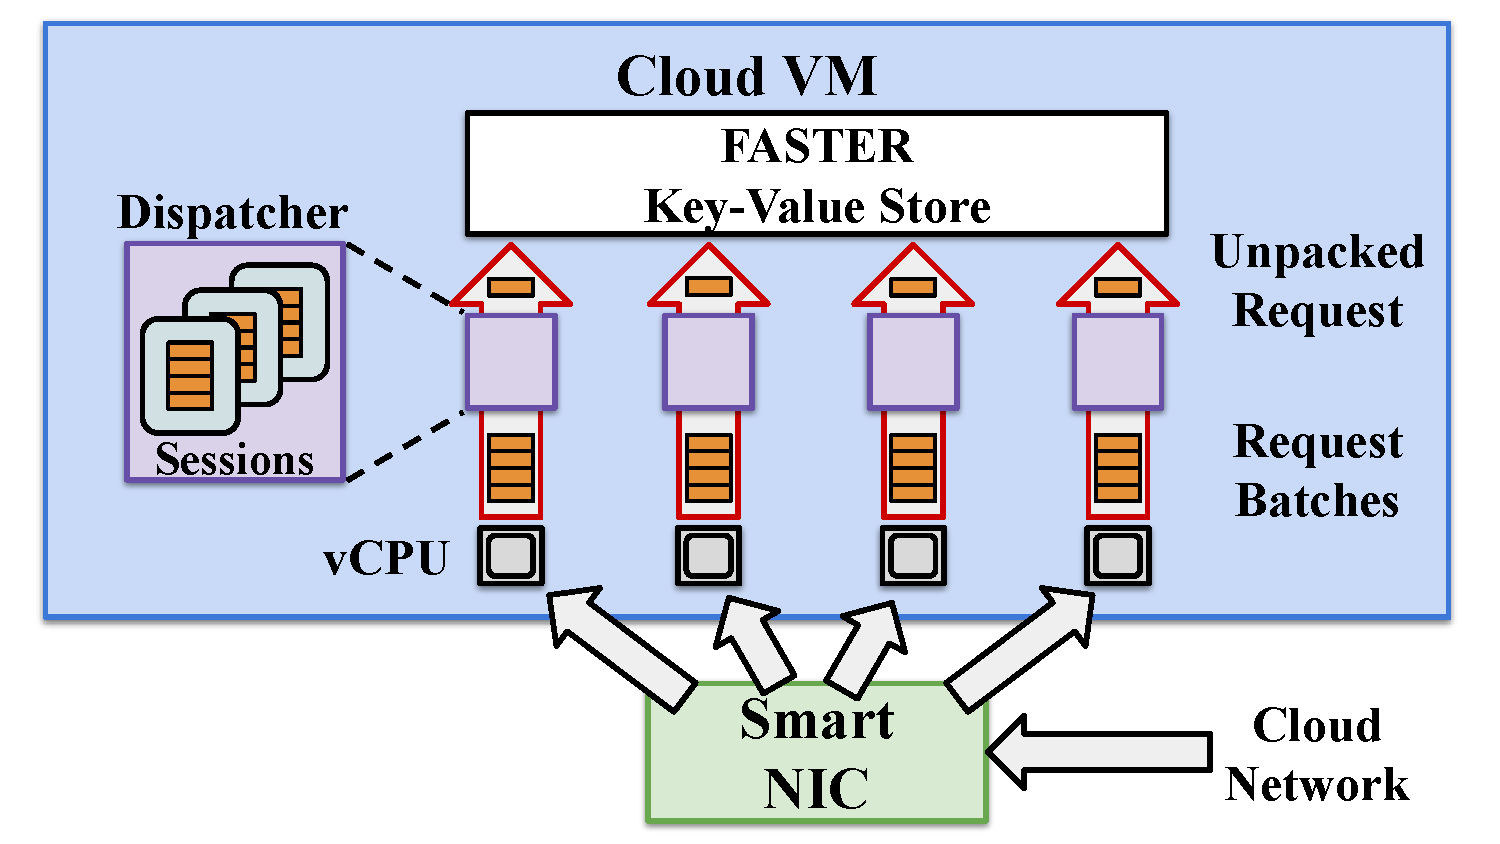
\includegraphics[width=0.9\columnwidth]{figures/server.pdf}
\caption{Each server thread receives batches of requests from sessions
    and processes them via a shared, per-machine \faster instance.
    Results are returned over the network by the same
    thread, avoiding cross-thread coordination.}
\label{fig:server}
\end{figure}


Shadowfax's network request dispatching mechanism and client library need to be
capable of saturating servers inside \faster.
%
One option would be to maintain a \faster instance per server thread,
partitioning records across them to avoid cache coherence costs.
%
However, this would create a routing problem at the server; requests
picked up from the network would need to be routed to the correct thread.
%
This would require cross-thread coordination, hurting throughput and
scalability.
%
Clients could be made responsible for routing requests to the correct
server thread, but this would require every client thread to open a
connection to every server thread and would not scale.
%
To avoid this, client threads could partition and shuffle requests between
themselves to directly transmit requests to the correct server thread, but this would
require cross-thread coordination at the client which would also not scale well.

Using a connectionless transport like UDP could make client side routing
feasible without introducing cross-thread coordination~\cite{fb-memcache,mica}.
%
However, the system would lose its ability to perform congestion
control and flow control, or tolerate packet loss, which
are basic requirements for running a
networked storage system.

Shadowfax avoids cross-thread coordination by sharing a single
instance of \faster between server threads.
%
\faster defers cross-core communication to hardware cache coherence on the
accessed records themselves, cleanly partitioning the rest of the system
(Figure~\ref{fig:server}).
%
Each server runs a pinned thread on each vCPU inside a cloud VM.
%
Each server thread runs a continuous loop that does two things.
%
First, it polls the network for new incoming connections.
%
Next, it polls existing connections for requests, and it unpacks these
requests, calling into \faster to handle each of them.
%
After requests are executed, the returned results are
transmitted back over the session they were received on.
%
Since \faster is shared, neither requests nor results are ever passed across
server threads.

\subsubsection{Client Sessions}
\label{sec:sessions}

\begin{figure}[t]
\centering
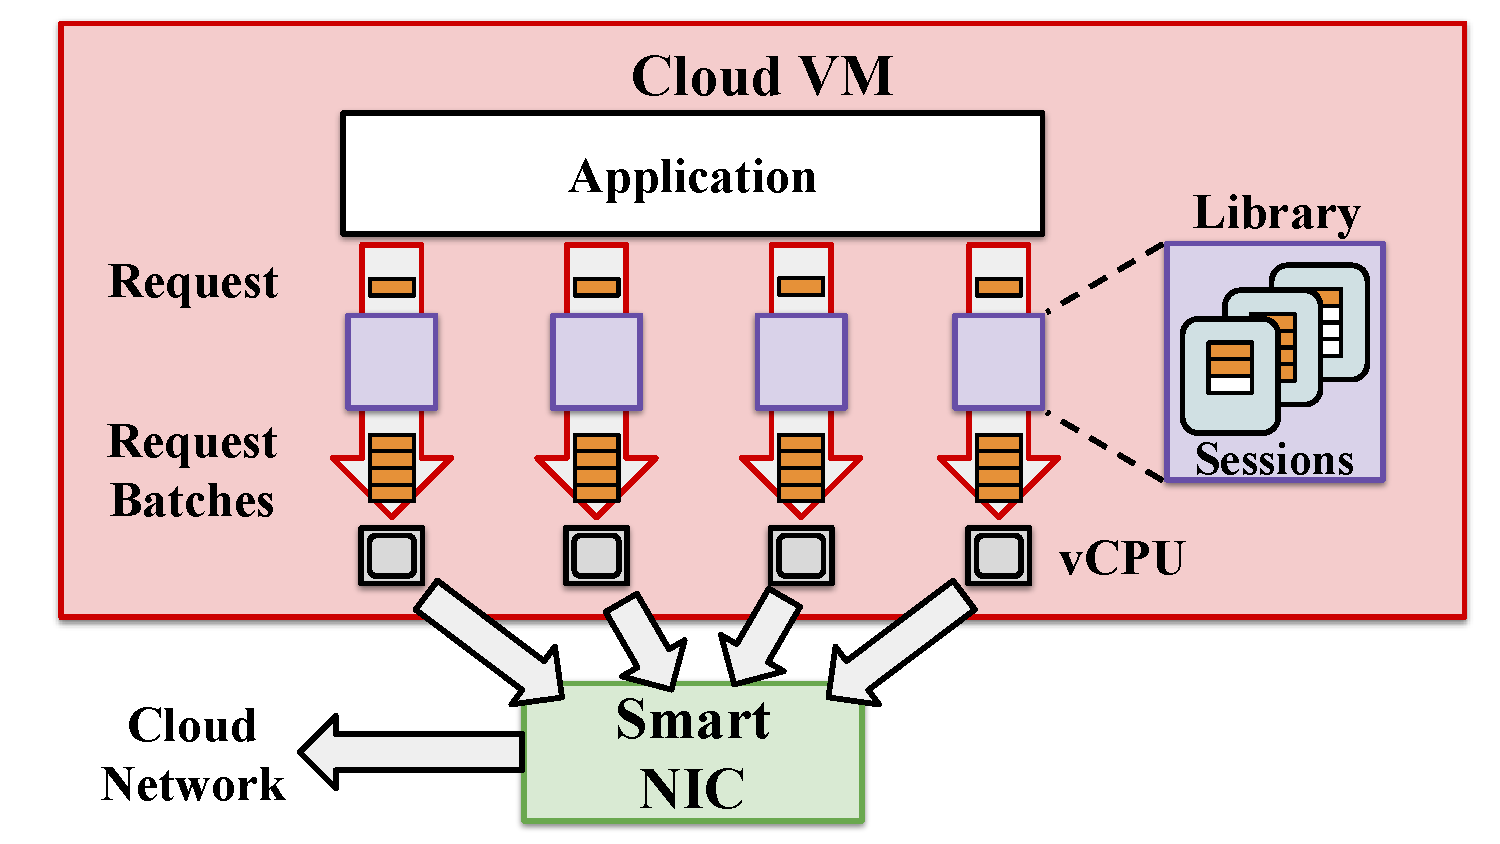
\includegraphics[width=0.9\columnwidth]{figures/client.pdf}
\caption{Client threads partition requests into per-session transmit buffers
  along with a callback.  Batches of asynchronous requests are kept pipelined
  to the server, keeping both the client and the server busy.}
\label{fig:client}
\end{figure}


Shadowfax's partitioned dispatch/shared data approach also extends to
clients.
%
Since they don't need to route requests to specific server threads, they
can reduce connection state while avoiding cross-thread coordination.

However, clients must also avoid stalling due to network delay in order to
saturate servers.
%
To do this, each client thread is pinned to a different vCPU of a cloud VM,
and it issues asynchronous requests against an instance of
Shadowfax's client library (Figure~\ref{fig:client}).
%
The library pipelines batches of these requests to servers.

The client library achieves this through \emph{sessions}.
%
When the library receives a request, it first checks if it has a
connection to the server that owns the corresponding record.
%
If it does not, it looks up a cached copy of ownership mappings
(periodically refreshed from the metadata store), establishes a
connection to a thread on the server that owns the record, and
associates a new \emph{session} with the connection.
%
Next, it buffers the request inside the session, enqueues a
completion callback for the request inside the session, and returns.
%
This allows the client thread to continue issuing requests without
blocking.
%
Once enough requests have been buffered inside a session, the
library sends them out in a batch to the server thread.
%
On receiving a batch of results from the server, the library
dequeues callbacks and executes them to complete the corresponding
requests.

Sessions are fully pipelined, so multiple batches of requests can be sent to a
server thread without waiting for responses.
%
This also means that a
client thread can continue issuing asynchronous requests into session
buffers while waiting for results.
%
This pipelined approach hides network delays and helps saturate servers.
%
It also helps keep request batch sizes small, which is good for latency.

%
% This approach to enqueuing and dequeuing callbacks assumes that server
% threads execute requests in a strict FIFO order.
%
% However, \faster executes requests for records on local SSD
% out-of-order.

\subsubsection{Exploiting Cloud Network Acceleration}

The cloud network has traditionally not been designed for high data
rates and efficiency.
%
The high CPU cost of processing packets over this network can easily
prevent servers and clients from retaining \faster's throughput.
%
However, this is beginning to change; many cloud providers are now
transparently offloading parts of their networking stack onto SmartNIC
FPGAs to reduce this cost.
%
Shadowfax's design interplays well with this acceleration; batched requests
avoid high per-packet overheads and its reduced connection count avoids the
performance collapse some systems experience~\cite{farm-2014}.

Since threads do not communicate or synchronize, all CPU cycles
recovered from offloading the network stack can be used for executing
requests at the server and issuing them from the client.
%
This allows Shadowfax to retain \faster's high throughput using the Linux
kernel's TCP stack on cloud networks, avoiding dependence on kernel-bypass
or RDMA.

\subsection{Record Ownership}
\label{sec:ownership}

To support distributed operations such as scale out and crash recovery,
Shadowfax must be able to move ownership of records between servers at
runtime.
%
This creates a problem during normal operation:
%
a client might send out a batch of requests to a server after referring
to its cache of ownership mappings.
%
By the time the server receives the batch, it might have lost ownership of
some of the requested records in the batch (e.g.\ due to scale out).
%
To solve this, the server must validate that it still owns the records requested
in the batch before it processes the batched requests.
%
This can hurt normal case throughput if each request in the
batch must be cross-checked against a set of hash ranges owned by the server.

Shadowfax solves this by associating the set of hash ranges owned by a server
with a per-server strictly-increasing \emph{view number}.
%
All request batches are tagged with a view number, letting servers quickly
assess whether the batch only includes requests for records that it currently owns.
%
When a server's set of owned ranges changes, its view number
is advanced.
%
Each server's latest view number is durably stored along with a list of the
hash ranges it owns in the metadata store.

When a client connects to a server, it caches a copy of the server's
latest view (a view number and its associated hash ranges) inside the session.
%
Every batch of requests sent on that session is tagged with this view number,
and clients only put requests for keys into batches that were owned by that
server in that view number.
%
%The server maintains a copy of its latest view too (periodically
%refreshed).
%
Upon receiving a batch, the server always checks its current view number
against the view number tagged on the batch.
%
If they match, then the server and client agree about what hash ranges are
owned by the server, ensuring the batch is safe to process without further key
or hash range checks on each request.
%
If they don't match, then either the client or the server has out-of-date
information about what hash ranges the server owns.
%
In this case, the server rejects the batch and refreshes its view from the
metadata server.
%
Upon receiving this batch rejection, the client refreshes its view information
from the metadata server and then reissues requests from the rejected batch.

In essence, view numbers offload expensive hash range checks on each requested
key to clients, reducing load at servers.
%
For a server that owns $P$ hash ranges accepting $R$ requests in batches of
size $B$, views reduce the cost of ownership checks from $O(R\log{P})$
to $O(R/B)$.
%
Even more crucially, since it is a single integer comparison per batch, it
ensures we never take a cache miss to perform record ownership checks, which would be prohibitive at 100~Mops/s.
%
Hence, views are key in supporting dynamic movement of ownership between
servers while preserving normal case throughput.
%
% Views also provide a means for lazily propagating ownership
% changes across the system;
%
% machines not involved in an ownership change can continue operating
% normally until they refresh their ownership cache.

% RS: I started writing this here before I realize the next section basically
% addresses this. Leaving it here in case I want to steal things from it.
%
%For consistency, all server threads must agree where in the sequence of the
%server's operations an old view ends and a new view begins to take effect.
%%
%However, a server's operations are not totally ordered, and we want to avoid
%pausing server threads on view transitions to bring them into agreement about
%hash range ownership.
%%
%View changes use the global cut mechanism used in other places in \faster that
%require propagating state changes among server threads; hence, for a short
%window on the server different threads may operate in different views.

\subsubsection{Ownership Transfer}
\label{design:ownership-tx}

When ownership of a hash range needs to be transferred to or away from a
server, its ownership mappings are first atomically updated at the
metadata store.
%
This increments its view number and adds or removes the hash range from
its mapping.
%
Servers and clients observe this view change either when they refresh
their local caches of views and ownership mappings (via an epoch action) or
when they communicate with a machine that has already observed this change.

When a server involved in the transfer observes that its view has
changed, it must move into the new view.
%
However, this step is not straightforward; keeping with
Shadowfax's design principle, it must be achieved without stalling
server threads.
%
\begin{figure}[t]
\centering
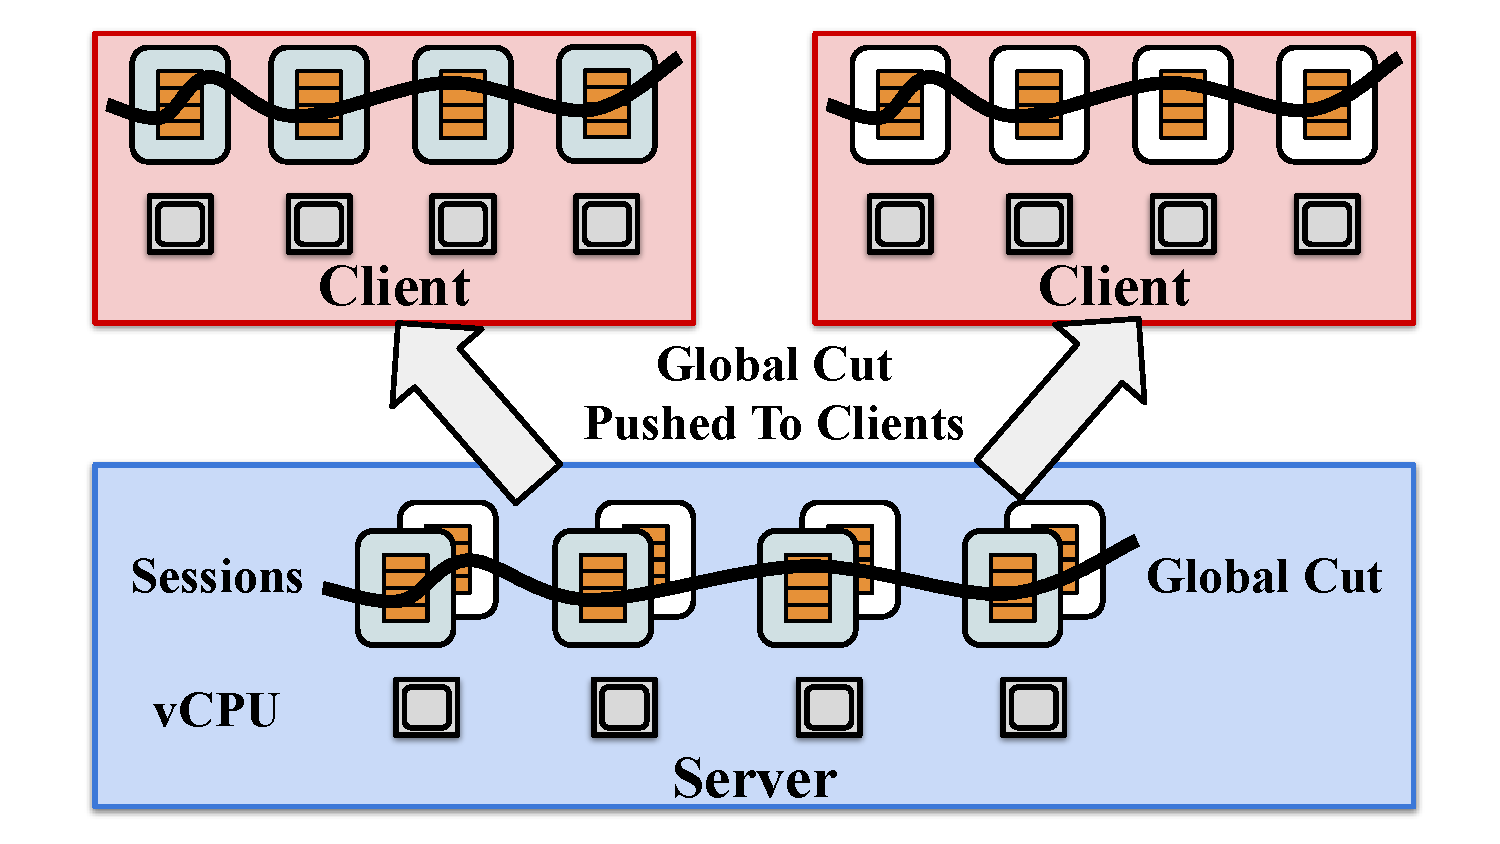
\includegraphics[width=\columnwidth]{figures/ownership-transfer.pdf}
\caption{Ownership transfer. A view change is asynchronously propagated
  within a server, defining a cut across server threads. Then, the server
  extends this into a global cut covering all its connected client sessions.
  This defines a global view boundary among all operations while
  avoiding cross-core coordination both at servers \emph{and} clients.}
\label{fig:ownership}
\end{figure}

%
%
Within the server, this view change is propagated asynchronously across
threads via an epoch action (Figure~\ref{fig:ownership}).
%
Threads each mark a point in their sequence of operations, collectively creating
an async cut among all of the operations on all of the threads at the server
(\S\ref{sec:epochs}).
%
This cut unambiguously ensures no two servers concurrently
serve operations on an overlapping hash range.
%
This approach is free of synchronous coordination, helping maintain high
throughput.

The server might be connected to clients still using the old view; it must also
propagate the view change to clients in a similar way without stalling client
threads.
%
Sessions help Shadowfax achieve this.
%
%Recall that a session is a mechanism for sending out asynchronous
%request batches, and associates with a connection between a server
%thread and a client thread.
%
When a server thread moves into a new view, view validations on request
batches received over sessions with clients still in an older view
are rejected.
%
%These rejections (and hence the view change) are propagated over
%the sessions to all client threads connected to the server thread.
%
% This effectively pushes the async cut taken on the server out to all
% clients connected to it.
%
On receiving a rejected batch over a session, each client thread first
independently updates its thread local cache of ownership mappings and
views.
%
Next, the thread marks the point in the sessions' sequence of
operations after which batches were rejected by the server (since there
can be multiple such batches because of pipelining, this has to be
the earliest such point).
%
Collectively, these points help create an implicit async cut across
threads within a
client.
%
Thus, clients avoid cross-thread
coordination when observing an ownership change.
%
Each client connected to the server creates its async cut independently,
resulting in a cluster wide \emph{asynchronous global cut} for ownership
transfer.

Once it has observed ownership transfer, each client thread must reissue
requests that were rejected by the previous owner.
%
It does so by \emph{shuffling} these requests between its sessions to the
previous and new owners of the transferred hash range.
%
First, they are marked invalid within the previous session's
buffer.
%
Next, they are (re)buffered into the correct session based on
the updated ownership mappings.

\section{Scale-Out and Hash Migration}
\label{sec:scale-out}

Sessions and view numbers help retain high throughput over the network,
but only upto a certain point.
%
Beyond high single node throughput, Shadowfax must also scale-out to
multiple servers, and it must retain \faster's throughput on each
of these servers.

In a distributed setting, partitioning becomes critical to
performance; it is well known that pre-partitioning records between
servers results in load imbalances, which significantly hurts
throughput~\cite{dynamo,slicer}.
%
Therefore, in order to meet its performance goals, Shadowfax must be
capable of dynamically migrating arbitrary, fine-grained splits of its
hash space between servers (new or existing) in response to load
imbalances.

For migration to be practical, it must have low impact on
throughput, and it must be fast.
%
Partitioned sessions help achieve the latter; they allow servers to
collect, transmit, receive and insert migrated records without
cross-thread coordination.
%
Since \faster is shared, server threads can also
easily interleave migration work with request processing.
%
Views help too; a server can own many fine-grained splits and still
serve 100~Mops/s during normal operation.

Achieving low impact during migration is harder.
%
Ownership of records must be safely moved between servers,
requests must be correctly executed on these records, and progress must
be tracked.
%
All of these could potentially introduce serial bottlenecks, and must
hence be carefully performed in an asynchronous, low-coordination way.
%
Shadowfax's migration protocol uses global cuts to proceed in
asynchronous phases
that transfer hash range ownership before migrating
records, as described next.

\subsection{Migration Protocol}

Shadowfax migrates hash ranges from a \emph{source} to a \emph{target} server.
%
Migration is implemented as a state machine on the source and target.
%
Both servers transition through migration phases on global cuts, created in the
same non-blocking, low-coordination way described in \S\ref{sec:epochs}.
%
First, each thread enters into a phase at a point in the sequence of requests
that it is processing that it chooses (a point that makes up part of the global
cut for the transition into that phase), and then it starts performing the work
of that phase.
%
Once all threads have entered into the phase and have completed all work
relating to it, the server transitions to the next phase.

Migration is driven by the source as we outline below (Figure~\ref{fig:source}):
%
%Its state machine (Figure~\ref{fig:source}) triggers the source to move into
%the new view, sampling and shipping of hot records to the target along with
%ownership transfer notification, and migration of records from the moved hash
%ranges to the target.
%
%We outline the source's phases below:% (Figure~\ref{fig:source}):

\begin{figure}[t]
\centering
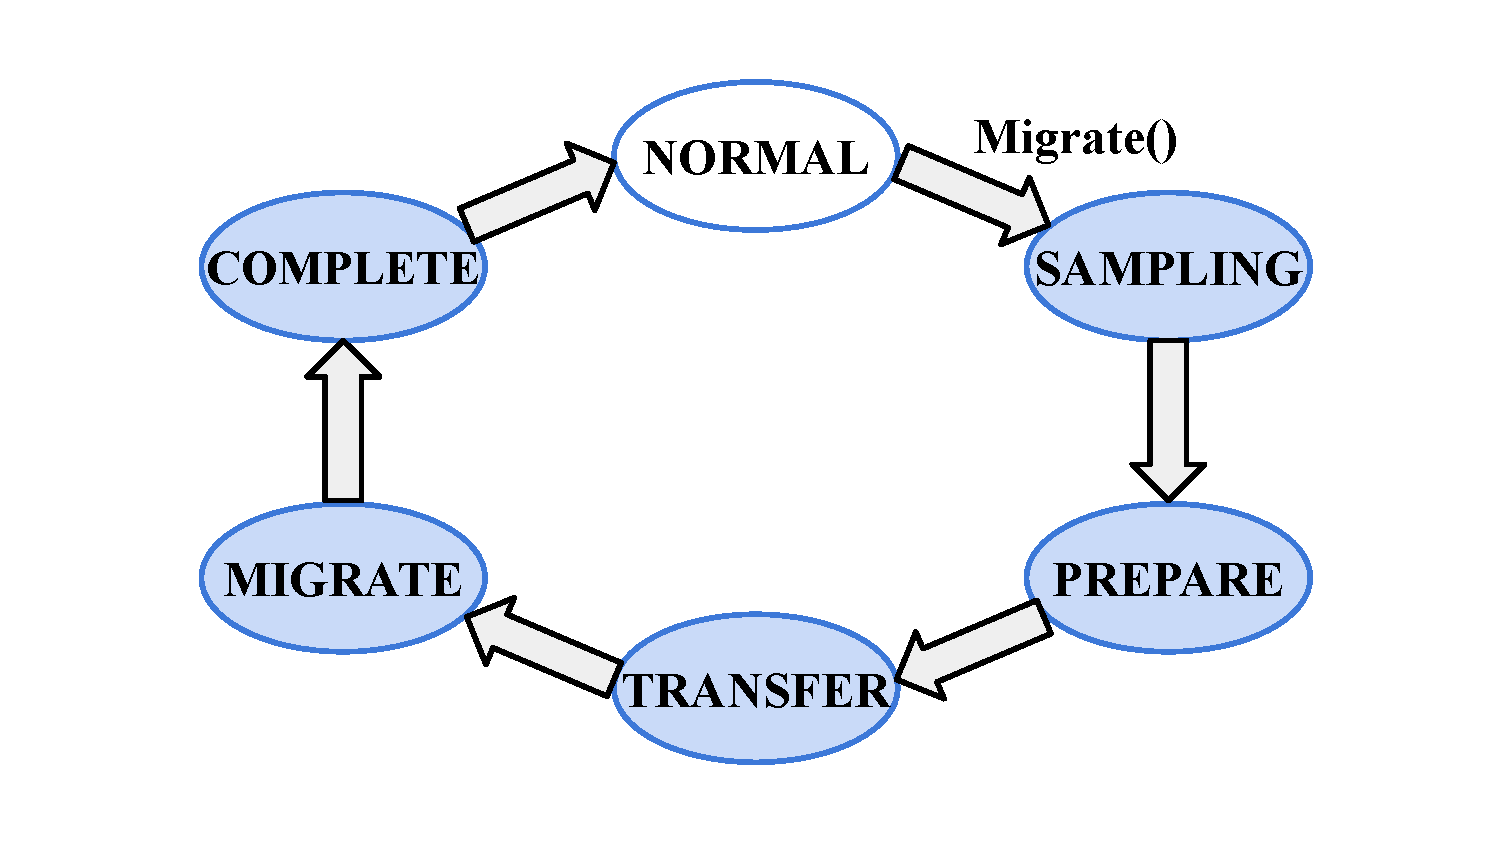
\includegraphics[width=\columnwidth]{figures/source.pdf}
\caption{Migration state machine on the source. This state machine is
    responsible for
    moving the source into the new view, for sampling and shipping hot records to the target, and for migrating all
    records in the hash range to the target.}
\label{fig:source}
\end{figure}


\begin{description}
\item[Sampling:]
Initiated by receiving a \texttt{Migrate()} RPC from a client, whereupon the source
\begin{enumerate}
  \item atomically remaps ownership of hash ranges from the source to the
    target, increments the source's and target's view numbers, and registers a
    dependency between the source and target (for crash recovery,
    \S\ref{sec:fault-tolerance}) within the metadata store;
  \item begins sampling hot records by forcing all accessed
    records to be copied to the \hlog tail.
\end{enumerate}

Since the records are not yet at the target and a migration is in
progress, both the source and the target continue to temporarily operate in the
old ownership view; at this point the source is still servicing requests for
records in the migrating ranges.
%
To ensure that sampled records only get copied once, the source only copies
records whose address is lower than the \hlog tail address at the start of this
phase.

\item[Prepare:]
Initiated after all source threads have completed the Sampling phase.
%
The source sends a \texttt{PrepForTransfer()} RPC to the target asynchronously,
transitioning the target to its own Target-Prepare phase.
The Target-Prepare phase tells the target that ownership transfer is
imminent. The target temporarily pends requests in the migrating hash
ranges (since some clients may discover the new views) and
services them after the source indicates that it has stopped servicing
requests in the old view.

\item[Transfer:]
Initiated after all source threads have completed the Prepare phase.
%
The source moves into its new view and stops servicing requests on the
migrating hash ranges.
%
When all server threads are in the new view, it sends out a
\texttt{TransferedOwnership()} RPC to the target asynchronously, which also
includes the hot records sampled in the Sampling phase.
%
This moves the target into its Target-Receive phase, whereupon it inserts the sampled
records into its \faster instance and then begins servicing requests for
the migrating hash ranges.
%
This also triggers the target to service any requests pending from the
Target-Prepare phase.

\item[Migrate:]
Initiated after all source threads have completed the Transfer phase.
%
The source uses thread-local sessions to send records in the migrating hash ranges
to the target.
%
Threads interleave processing normal requests with sending batches of migrating
records collected from the source's hash table to the target.
%
Each thread works on independent, non-overlapping hash table regions, avoiding
contention.

\item[Complete:]
Initiated after all source threads have completed the Migrate phase.
%
The source sends a \texttt{CompleteMigration()} RPC asynchronously, moving the target to the Target-Complete phase.
%
Then,
% the source asynchronously checkpoints its log, so if it crashes
% after migration has completed, it can be recovered without filtering out
% migrated records.
%
% When the checkpoint completes,
the source sets a flag in the metadata store
indicating that its role in migration is complete, and it returns to
normal operation.

\end{description}

\iffalse
\begin{table}[t]
\small
\begin{tabular}[]{p{0.95\columnwidth}}
\toprule
\textbf{Scale Out Phases On The Source Server} \\
\midrule
\textbf{Sample} \\
  \hspace{1em} $\diamond$ Copy records to the tail of the log on first access \\
  \\
\textbf{Prepare} \\
  \hspace{1em} $\diamond$ Prepare Target for ownership transfer \\
  \hspace{2em} $\rightarrow$ \texttt{PrepForTransfer()} RPC to Target \\
  \hspace{1em} $\diamond$ Complete all pending requests \\
  \\
\textbf{Transfer} \\
  \hspace{1em} $\diamond$ Change view \\
  \hspace{1em} $\diamond$ Transfer ownership and sampled records to the Target \\
  \hspace{2em} $\rightarrow$ \texttt{TransferOwnership()} RPC to Target \\
  \\
\textbf{Migrate} \\
  \hspace{1em} $\diamond$ Move records to the Target in parallel \\
  \hspace{2em} $\rightarrow$ \texttt{PushHashes()} RPCs to Target \\
  \\
\textbf{Complete} \\
  \hspace{1em} $\diamond$ Inform Target that migration has completed \\
  \hspace{2em} $\rightarrow$ \texttt{CompleteMigration()} RPC to Target \\
  \hspace{1em} $\diamond$ Take a checkpoint \\
  \hspace{1em} $\diamond$ Set vote at the Metadata store \\
  \\
\bottomrule
\end{tabular}
\caption{}
\label{table:source}
\end{table}
\fi

\begin{figure}[t]
\centering
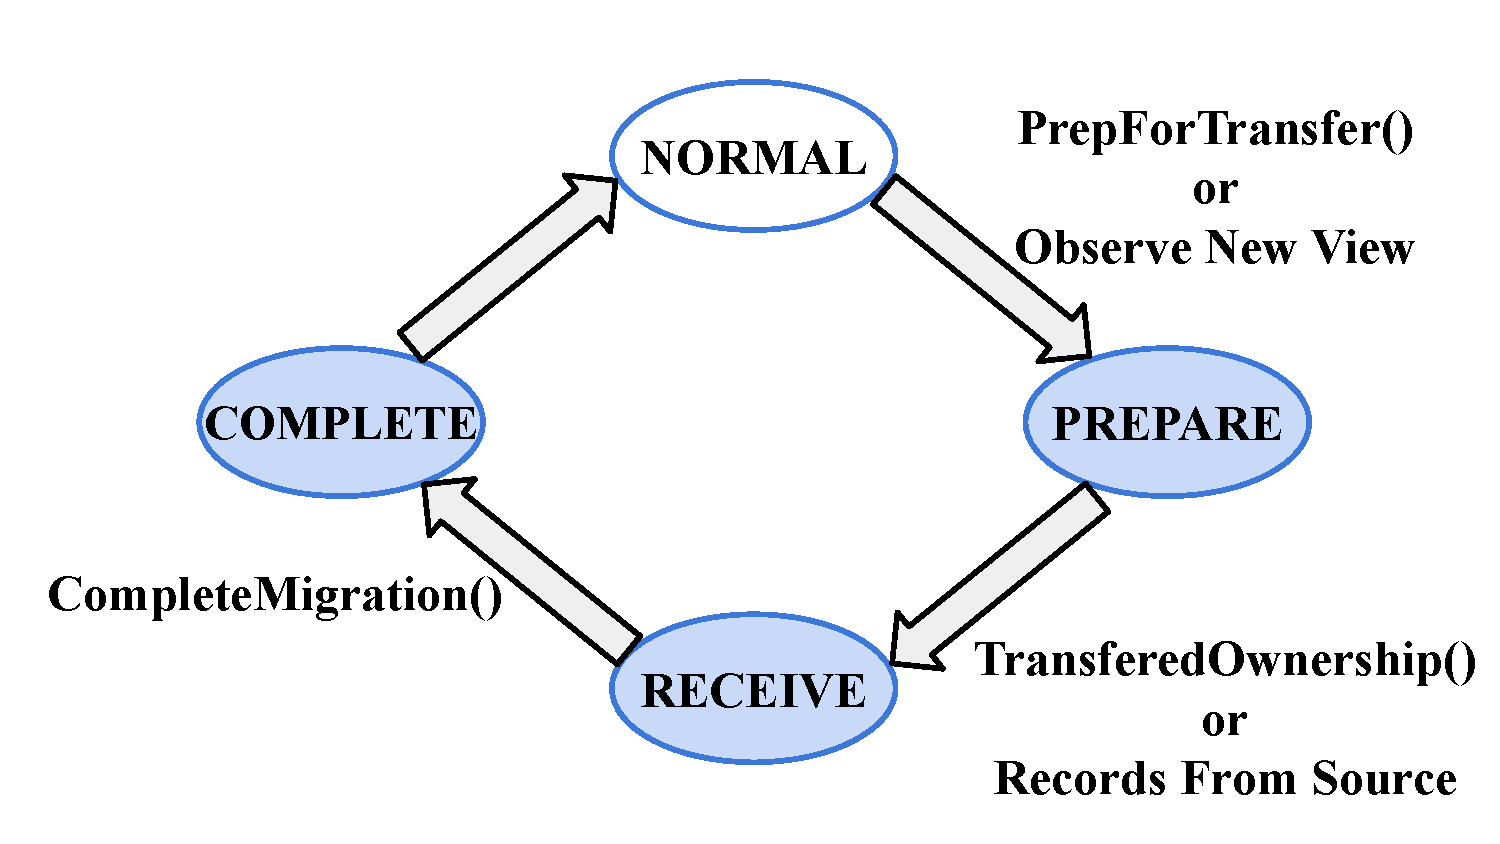
\includegraphics[width=\columnwidth]{figures/target.pdf}
\caption{Migration state machine on the target. It is
    responsible for moving the target into the new view,
    safely executing requests on the migrating hash
    range, and receiving records from the source}
\label{fig:target}
\end{figure}


The target is mostly passive during migration; most of its phase changes are
triggered by source RPCs (Figure~\ref{fig:target}).
%
Requests for a record may arrive after a \texttt{TransferredOwnership()} RPC is received by the target, but before the
source has sent that record.
%
The target marks these requests pending, and it processes them when it receives
the corresponding record.

When the target receives the \texttt{CompleteMigration()} RPC,
% it also
% takes an asynchronous checkpoint, ensuring that it can be recovered to its
% post-migration state in the case that the source or target crashes.
%
% Afterward,
it also sets a flag at the metadata store indicating that its role in the
migration is complete, and it returns to normal operation.

%
%Its state machine (Figure~\ref{fig:target}) is responsible for moving it
%into the new view, safely executing requests on the migrating hash
%range, and receiving records from the source.
%%
%It achieves all of this through the following phases:

%\begin{description}
%\item[Prepare:]
%The target enters into this phase on receiving a \texttt{PrepForTransfer()}
%RPC from the source.
%%
%During this phase, if it receives request batches from clients that are
%tagged with a new view, it refreshes its view from the metadata store
%and takes a global cut to propagate the new view. {\color{red} RS: Why?}
%%
%Occasionally, due to network delays, the target might observe an
%ownership change (either through clients or when it periodically
%refreshes its view) before
%it has received and processed a \texttt{PrepForTransfer()} from the
%source.
%%
%If this happens, it assumes that a migration will happen soon, enters
%into this phase on its own, and moves into its new view.
%
%\hspace{0.2cm}
%When processing a request during this phase, if the target finds that the
%key falls in the
%migrating hash range, it stops executing the request.
%%
%This is because there might be threads on the source still executing
%requests on the hash range.
%%
%Instead, it buffers the request
%inside the session it was received on.
%%
%To prevent head of line blocking at the client, the target returns a
%special result called \texttt{PENDING} along with a monotonic identifier
%for the request.
%%
%On receiving this result, the client dequeues the request's callback and
%moves it into a session local hashmap indexed by this identifier.
%%
%This way, clients can continue issuing asynchronous requests during
%migration without blocking on ownership transfer.

%\item[Receive:]
%The target enters into this phase on receiving a
%\texttt{TransferedOwnership()} RPC from the source.
%%
%If it hasn't already observed and entered into a new view, it does so
%now, following which it inserts all sampled records that were shipped
%with the RPC.
%%
%During this phase, the target receives batches of records from the
%source, which it inserts into its instance of \faster.
%%
%Occassionally, due to networking delays, the target might receive these
%batches from the source before the \texttt{TransferedOwnership()} RPC.
%%
%If this happens, it means that the source has entered into the
%\texttt{Migrate} phase on its state machine after moving into its new
%view.
%%
%As a result, the target can safely enter into this phase, and also move
%into its new view if required.
%%
%When the RPC does arrive, the target only inserts all sampled records
%that were shipped with it.

%\hspace{0.2cm}
%During this phase, the target can safely execute requests on the
%migrating hash range.
%%
%If it receives a request that attempts to read a record that has not
%been migrated yet, it reuses the \texttt{PREPARE} phases' buffering
%mechanism to avoid head of line blocking at the client.
%%
%Starting from this phase, the target also tries to clear out
%such requests by periodically re-executing tiny batches of them until
%there are none left.

%\item[Complete:]
%The target enters into this phase on receiving a
%\texttt{CompleteMigration()} RPC from the source.
%%
%Like on the source, the target first takes an asynchronous checkpoint to avoid rolling
%back migration if it crashes, and then sets a flag at the metadata
%store's migration dependency to indicate that its role is complete.
%%
%It then returns to normal operation.
%
%\end{description}

\iffalse
\begin{table}[t]
\small
\begin{tabular}[]{p{0.95\columnwidth}}
\toprule
\textbf{Scale Out Phases On The Target Server} \\
\midrule
\textbf{Prepare} \\
  \hspace{1em} $\diamond$ Buffer client requests on migrating hash range \\
  \\
\textbf{Receive} \\
  \hspace{1em} $\diamond$ Execute client requests on migrating hash range \\
  \hspace{1em} $\diamond$ Insert migrated records in parallel \\
  \\
\textbf{Complete} \\
  \hspace{1em} $\diamond$ Take a checkpoint \\
  \hspace{1em} $\diamond$ Set vote at the Metadata store \\
  \\
\bottomrule
\end{tabular}
\caption{}
\label{table:target}
\end{table}

\begin{table}[t]
\small
\begin{tabular}[]{p{0.95\columnwidth}}
\toprule
\textbf{Scale Out RPCs} \\
\midrule
\textbf{Migrate()} \\
  \hspace{1em} $\diamond$ Starts scale out on Source \\
  \hspace{1em} $\diamond$ Moves Source to \textbf{Sample} \\
  \\
\textbf{PrepForTransfer()} \\
  \hspace{1em} $\diamond$ Moves Target to \textbf{Prepare} \\
  \\
\textbf{TransferOwnership()} \\
  \hspace{1em} $\diamond$ Transfers ownership
    and sampled records to Target \\
  \hspace{1em} $\diamond$ Moves Target to \textbf{Receive} \\
  \\
\textbf{PushHashes()} \\
  \hspace{1em} $\diamond$ Sends batch of records to Target \\
  \hspace{1em} $\diamond$ If needed, moves Target to \textbf{Receive} \\
  \\
\textbf{CompleteMigration()} \\
  \hspace{1em} $\diamond$ Moves Target to \textbf{Complete} \\
  \\
\bottomrule
\end{tabular}
\caption{}
\label{table:rpc}
\end{table}
\fi

Migration has succeeded once both servers have set their respective
flags at the metadata store.
%
A cluster management thread will have to periodically check these flags;
%
on finding both set, it deletes the
dependency at the metadata store to complete migration.

Shadowfax maintains high throughput during
scale up via low-coordination, non-blocking
epoch actions and purely asynchronous inter-machine communication.
%
The source prioritizes request processing, making progress in between request batches.
%
Its state machine transitions are independent of the target; all
migration RPCs and checkpoints are asynchronous.
%
The target prioritizes request processing in the same way.
%
Early ownership transfer, sampled records, and pending operations
let the target start servicing requests on moved ranges
quickly, improving throughput recovery.
%
Sessions let the source collect and
asynchronously transmit records in parallel while the target receives
and inserts them in parallel.

% Finally, the protocol is also wait-free; if either the source or target
% fail to make progress through it, an independent entity can always set a
% cancellation bit at the metadata store's migration dependency and roll
% back both servers.

\subsection{Leveraging Shared Storage for Decoupling}
\label{sec:design:indirection}

Migration cannot complete until all records have been
moved to the target, so Shadowfax must ensure that this
happens quickly.
%
However, \faster's larger-than-memory index makes this challenging:
entries in its hash table point to linked lists of records, which can
span onto local SSD.
%
Performing I/O (sequential or random) to migrate these records
can slow migration and hurt throughput.

Shadowfax's shared remote tier helps solve this problem.
%
Records on local SSD are always eventually flushed to this tier, so migration
can avoid accessing them.
%
When the source encounters an address for a record in a list that is on the
SSD, it sends an \emph{indirection record} to the target that indicates this
record's location in the shared tier.
%
This indirection record contains the next address in the list, an identifier for the
source's log, the hash range being migrated, and the hash entry that
pointed to the list.
%
The target inserts these records into its hash table using the hash
entry contained in the record.
%
% These records become part of its end-of-migration checkpoint.
%
Overall, these fine-grained inter-log dependencies represented by indirection
records accelerate migration completion by eliminating all I/O
that would otherwise be needed to consolidate records and transmit them
to the target.

During normal operation, if the target encounters an indirection record
when processing a request and the request's key falls in the
hash range contained in the record, the target asynchronously retrieves
the actual record from the
shared tier using the contained address and log identifier, inserts it
into its hash table, and then completes the request.

\subsection{Cleaning Up Indirection Records}

\begin{figure}[t]
\centering
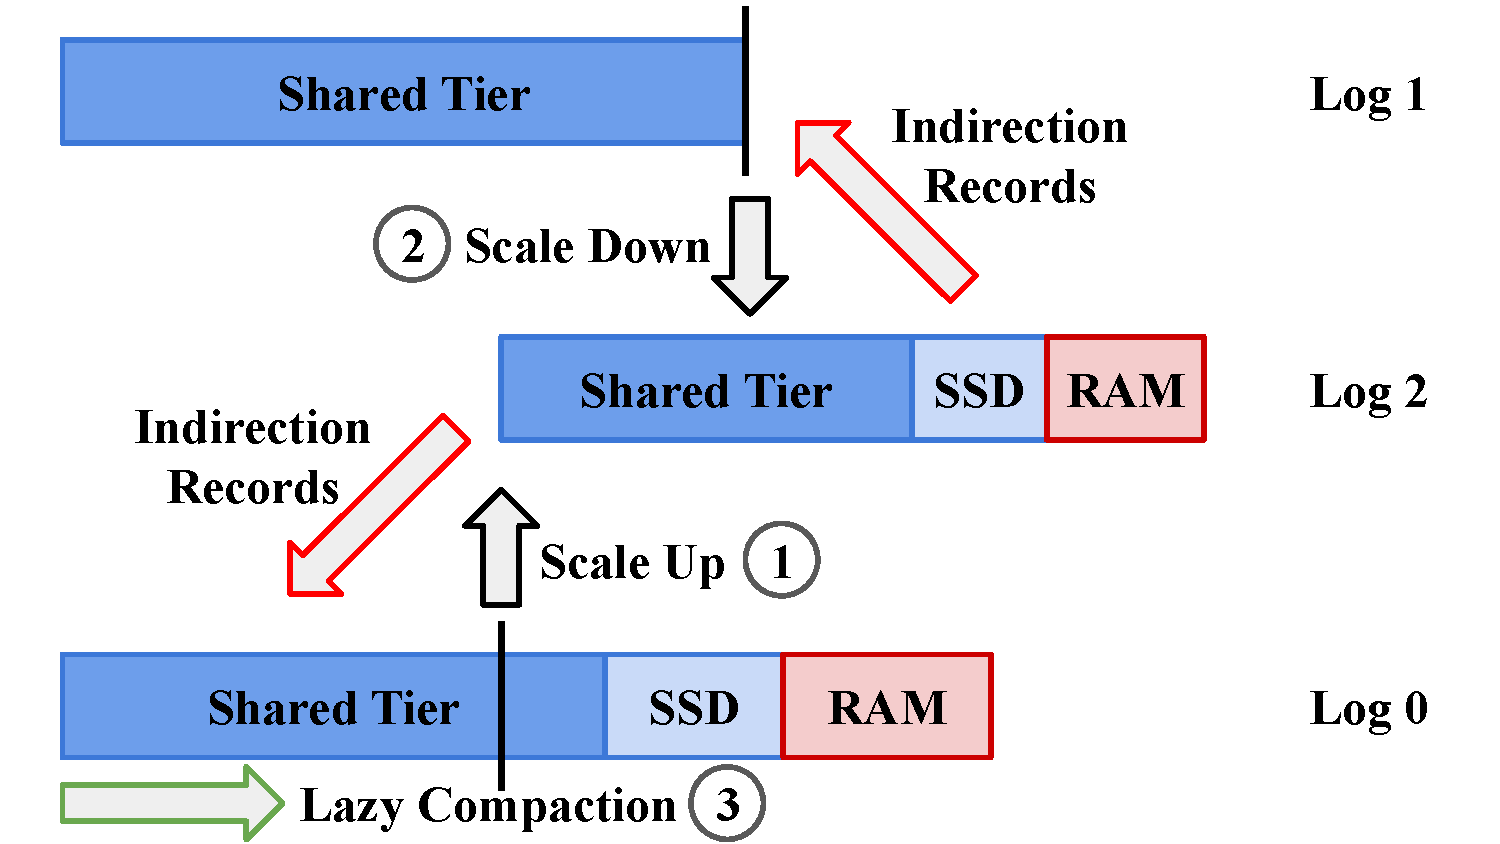
\includegraphics[width=\columnwidth]{figures/indirection.pdf}
\caption{Indirection records create fine-grained data dependencies
    between logs. These dependencies are cleaned up lazily during
    log compaction.
%    This allows migration to be restricted to
%    main memory.
}
\label{fig:dfs}
\end{figure}


Migrations can accumulate indirection records between server logs
for records that are never accessed (Figure~\ref{fig:dfs}).
%
On scaling up (\one) by moving a hash range from
Log~0 to Log~2, Log~2 contains indirection records that point to
Log~0 on the shared tier.
%
Dependencies are also created during scale down (\two) when
records on Log~1 are migrated to Log~2.
%
These dependencies must eventually be cleaned up.

Shadowfax must already periodically do log compaction to eliminate stale
versions of records from its shared tier; resolving and removing indirection
records can be piggybacked on this process to eliminate overheads for
cleaning them (\three).
%
When compacting its log, if a server encounters a record belonging to a
hash range it no longer owns, the server transmits the record to the
current owner.
%
On receiving such a record, the owner first looks up the key.
%
If it encounters an indirection record while doing so and the key falls
in the contained hash range, then it means that the key was not retrieved
from the shared tier after migration.
%
In this case, the server inserts the received record; otherwise, it discards
the record.

Barring normal case request processing, this lazy approach
ensures that records not in main memory are accessed only once, during
the sequential I/O of compaction, which has to be done anyway.
%
It is also deadlock-free:
%
two servers might have indirection records pointing to each others' log,
but the resulting dependencies are cleaned up independently.
